\documentclass{beamer}

\usetheme{CambridgeUS}

\title[MCTS]{CS4246 AI Planning and Decision Making}
\subtitle{Monte Carlo Tree Search in Texas Holdem' Poker}
\author[Davin Choo, Keng Kiat, Wang Zi]{Choo XianJun, Davin\inst{1}\\ \and Lim Keng Kiat\inst{1}\\ \and Wang Zi\inst{1}}
\institute[NUS]{ \inst{1} Department of Computer Science\\ National University of Singapore}
\subject{Computer Science}
\date{}

\begin{document}
  \frame{\titlepage}

  \section{Motivation}

  \begin{frame}
    \frametitle{Monte Carlo Tree Search}
    \begin{itemize}
        \item<1-> Why MCTS?
        \item<2-> Comparison against classic tree search algorithms
        \begin{itemize}
          \item $\alpha$-$\beta$ pruning
          \item $A^*$ search
        \end{itemize}
    \end{itemize}
  \end{frame}
  
  \section{Introduction to Monte Carlo Tree Search}
    
  \begin{frame}
      \frametitle{Overview}
      \begin{enumerate}
          \item<1-> Monte Carlo
          \begin{itemize}
            \item A statistical approach
          \end{itemize}
          \item<2-> Tree Search
          \begin{itemize}
            \item Search on a sequential problem domain
          \end{itemize}
      \end{enumerate}
  \end{frame}
  
  \begin{frame}
    \frametitle{The 4 MCTS Phases}
    \begin{enumerate}
        \item<1-5> Selection
        \begin{itemize}
          \item<1> While we are at a visited node, \textit{select} a child node
          \item<1> How? We shall discuss this later.
        \end{itemize}
        \item<2-5> Expansion
        \begin{itemize}
          \item<2> If we reach an unvisited node, \textit{expand}/create all possible child nodes
          \item<2> Mark node as visited and pick one of child nodes to explore
        \end{itemize}
        \item<3-5> Simulation
        \begin{itemize}
          \item<3> While we have not reached a terminal node, \textit{simulate} a playthrough/rollout
        \end{itemize}
        \item<4-5> Backpropagation
        \begin{itemize}
          \item<4> Compute reward at terminal node
          \item<4> \textit{Backpropagate} reward back towards the root
          \item<4> Update relevant details needed to make selection decisions
        \end{itemize}
    \end{enumerate}
  \end{frame}

  \begin{frame}
    \frametitle{MCTS Outline}
    \begin{figure}
        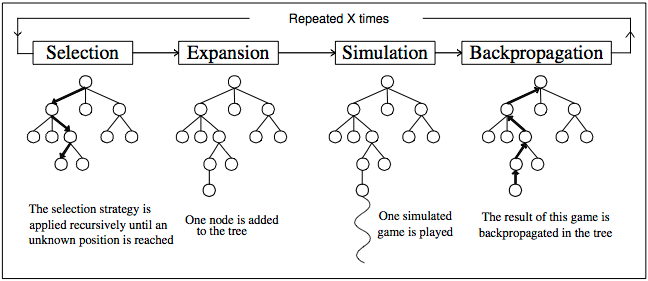
\includegraphics[width=\textwidth]{../MCTS_outline.png}
        \caption{Monte Carlo Tree Search outline from Chaslot (2010)}
    \end{figure}
  \end{frame}
  
  \section{MCTS Details}
  
  \begin{frame}
    \frametitle{Selection Choices}
    \begin{itemize}
      \item<1-> Exploration vs. Exploitation
      \item<2-> Upper Confidence Bound (UCB1)
      $$UCB1 = \overline{X}_j + \sqrt{\frac{2 \ln n}{n_j}}$$
      \item<3-> Upper Confidence Bound for Trees (UCT)
      $$UCT = \overline{X}_j + 2C_p\sqrt{\frac{2 \ln n}{n_j}}$$
    \end{itemize}
  \end{frame}
  
  \begin{frame}
    \frametitle{Properties}
    \begin{itemize}
      \item<1-> Ahueristic
      \begin{itemize}
        \item Compared to other classical search algorithms that need intermediate evaluation functions/heuristics
      \end{itemize}
      \item<2-> Anytime
      \begin{itemize}
        \item Able to make sense even if stopped halfway during computation
      \end{itemize}
      \item<3-> Asymmetric
      \begin{itemize}
        \item Favour more promising nodes
      \end{itemize}
    \end{itemize}
  \end{frame}
  
  \begin{frame}
    \frametitle{Asymmetric Tree Growth}
    \begin{figure}
        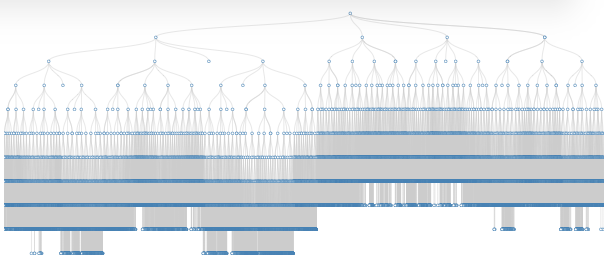
\includegraphics[width=\textwidth]{asymmetric.png}
        \caption{Illustration of asymmetric search tree of our MCTS Poker bot}
    \end{figure}
  \end{frame}

  \begin{frame}
    \frametitle{Extensions to MCTS}
    \begin{itemize}
      \item<1-> Parallelization
      \begin{itemize}
        \item Leaf/Root/Tree parallelization
      \end{itemize}
      \item<2-> Re-using search trees
      \begin{itemize}
        \item Start search tree for new node from appropriate branch of old node
      \end{itemize}
      \item<3-> Opponent Modelling
      \begin{itemize}
        \item Vanilla MCTS assumes uniform distribution over opponent's actions
      \end{itemize}
      \item<4-> Adaptive Play
      \begin{itemize}
        \item Able to detect change in opponent's strategy/playing style
      \end{itemize}
    \end{itemize}
  \end{frame}
  
  \section{Application}
    
  \begin{frame}
    \frametitle{2 Player Limit Texas Holdem' Poker}
    \begin{itemize}
      \item<1-> Rules
      \begin{itemize}
        \item Hand strength: Royal Flush $>$ Straight Flush $>$ Four of a Kind $> ... $
        \item Small blinds, Big blinds
        \item Actions: Fold, Check, Call, Raise (Small), Raise (Big)
        \item Stages: Deal, Flop, Turn, River
      \end{itemize}
      \item<2-> Properties
      \begin{itemize}
        \item Partially observable
        \item Non-deterministic
        \item Large belief space $\rightarrow$ We approximate with MCTS
      \end{itemize}
      \item<3-> Alternative approaches (Game theory, etc)
    \end{itemize}
  \end{frame}
  
  \begin{frame}
    \frametitle{Implementation}
    \begin{itemize}
      \item Python 2.7
      \item Demo
    \end{itemize}
  \end{frame}

  \section{The End}
  
  \begin{frame}
    \frametitle{Where can we go from here?}
    \begin{itemize}
      \item Look into MCTS extensions
      \item Extend our MCTS bot to Multiplayer No Limit Texas Holdem' Poker
      \item Hook up our MCTS bot with an actual Poker game client and see how well it fares
    \end{itemize}
  \end{frame}
  
  \begin{frame}
    \begin{itemize}
      \frametitle{Thank you for your time}
      \item For references and source codes, refer to report.
      \item Questions?
    \end{itemize}
  \end{frame}

\end{document}